\subsubsection{Gradientenindexprofil}

Bei polymer optischen Fasern mit Gradientenindexprofil (GI-POF) nimmt die
Brechzahl vom Mantel bis zur Mitte des Kerns kontinuierlich zu (linke Grafik in
\autoref{fig:pofgi}). Dadurch breitet sich das Licht sinusförmig in der Faser
aus (rechte Grafik in \autoref{fig:pofgi}).

Als Kernmaterial werden der Kunststoff CYTOP\textsuperscript{\texttrademark} der
Asahi Glass Company oder Polymethylmethacrylat verwendet \cite{pofacgif}. Der
Kerndurchmesser einer GI-POF beträgt ca. \nolbreaks{100 µm} und liegt damit bei
einem Zehntel des Kerndurchmessers einer SI-POF. Der geringere Kerndurchmesser
hat geringere Laufzeitunterschiede zur Folge; dies ermöglicht eine höhere
Frequenz der Lichtimpulse. Zudem ist die Dämpfung einer GI-POF mit unter
\nolbreaks{20 dB/km} (siehe \autoref{fig:pofgidaempfung}) erheblich geringer als
die Dämpfung einer SI-POF (ca. \nolbreaks{100 dB/km}).

Die Bandbreite von Fasern mit Gradientenindexprofil ist daher signifikant höher
als bei Fasern mit Stufenindexprofil. Es werden Durchsatzraten bis zu 40
Gigabit/s auf 100 m erreicht.

Aufgrund der hohen Bitraten und ihrer Biegsamkeit werden GI-POF vor allem in
\glqq Local Area Networks\grqq{} (LAN) und in Supercomputern eingesetzt.
\cite{poflee}

\ifthenelse{\boolean{showPics}}{
    \begin{figure}[h]
        \begin{center}
            \begin{minipage}[t]{0.55\textwidth}
                \begin{center}
                    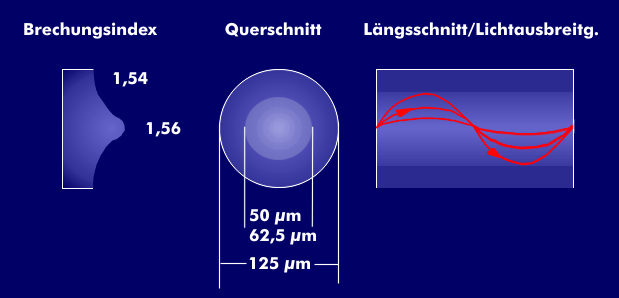
\includegraphics[height=0.1\textheight]{Bilder/Optische_Wellenleiter_Die_Polymer_Optische_Faser/Brechzahlprofile/pofgi.png}
                    \caption[Aufbau des Gradientenindexprofils \newline \url{http://www.itwissen.info/bilder/aufbau-und-brechungsprofil-der-gradientenfaser.png} (zuletzt aufgerufen am 19.09.2015)]{Aufbau des Gradientenindexprofils}
                    \label{fig:pofgi}
                \end{center}
            \end{minipage}
            \hspace{0.025\textwidth}
            \begin{minipage}[t]{0.4\textwidth}
                \begin{center}
                    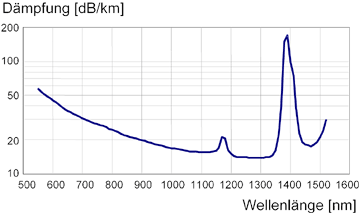
\includegraphics[height=0.1\textheight]{Bilder/Optische_Wellenleiter_Die_Polymer_Optische_Faser/Brechzahlprofile/pofgidaempfung.png}
                    \caption[Vergleich der Dämpfungswerte von GI-POF und SI-POF \newline \url{http://www.pofac.fh-nuernberg.de/pofac/de/was_sind_pof/images/gradientenindex_daempfung.png} (zuletzt aufgerufen am 19.09.2015)]{Vergleich der Dämpfungswerte von GI-POF und SI-POF}
                    \label{fig:pofgidaempfung}
                \end{center}
            \end{minipage}
        \end{center}
    \end{figure}
}{}
